%!TEX root = ../main.tex

\section{Germanium}
\label{sec:germanium}

Bei der ersten untersuchten Probe handelt es sich um einen konventionellen Germanium-
Halbleiter der mittels elektrolytischer Goldkontakte und -drähte an die Messapperatur
angeschlossen ist. Das Germanium-Plättchen hat, wie in \autoref{fig:germanium} 
gezeigt, die Ausmaße H$\times$W$\times$L = $\SI{1}{\milli\meter}\times\SI{10}{\milli
\meter}\times\SI{19}{\milli\meter}$. Im Folgenden sollen nun einige elektronische
Eigenschaften in Abhängigkeit der Temperatur des Halbleiters diskutiert werden.

\begin{figure}
	\centering
	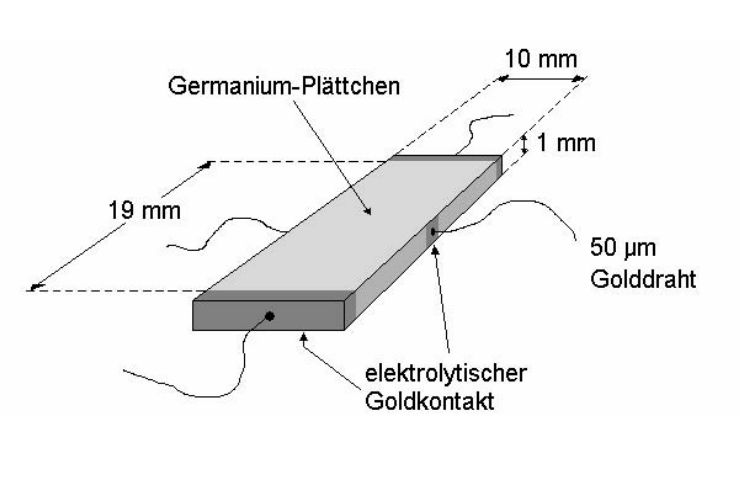
\includegraphics[width=1.0\textwidth]{./fig/germanium.png}
	\caption{Schematische Darstellung der Germanium Probe. Abbildung entnommen 
aus \cite{Manual}}
	\label{fig:germanium}
\end{figure}

\subsection{Leitfähigkeit und Hallkoeffizient}
\label{ssec:leitfähigkeit}

Die Leitfähigkeit $\sigma$ sowie der Hallkoeffizient $R_\text{Hall}$ werden wie in 
\autoref{chap:theory} dargestellt berechnet. Dabei ergeben sich über verschiedene
Temperaturen die in \autoref{fig:measurement_A} und \autoref{fig:logarithmic_A} 
gezeigten Verläufe. Die gemessenen Spannungswerte, aus denen diese Größen berechnet 
sind sind dem Protokoll in    angehängt.

\begin{figure}
	\centering
	\begin{subfigure}[h]{0.45\linewidth}
	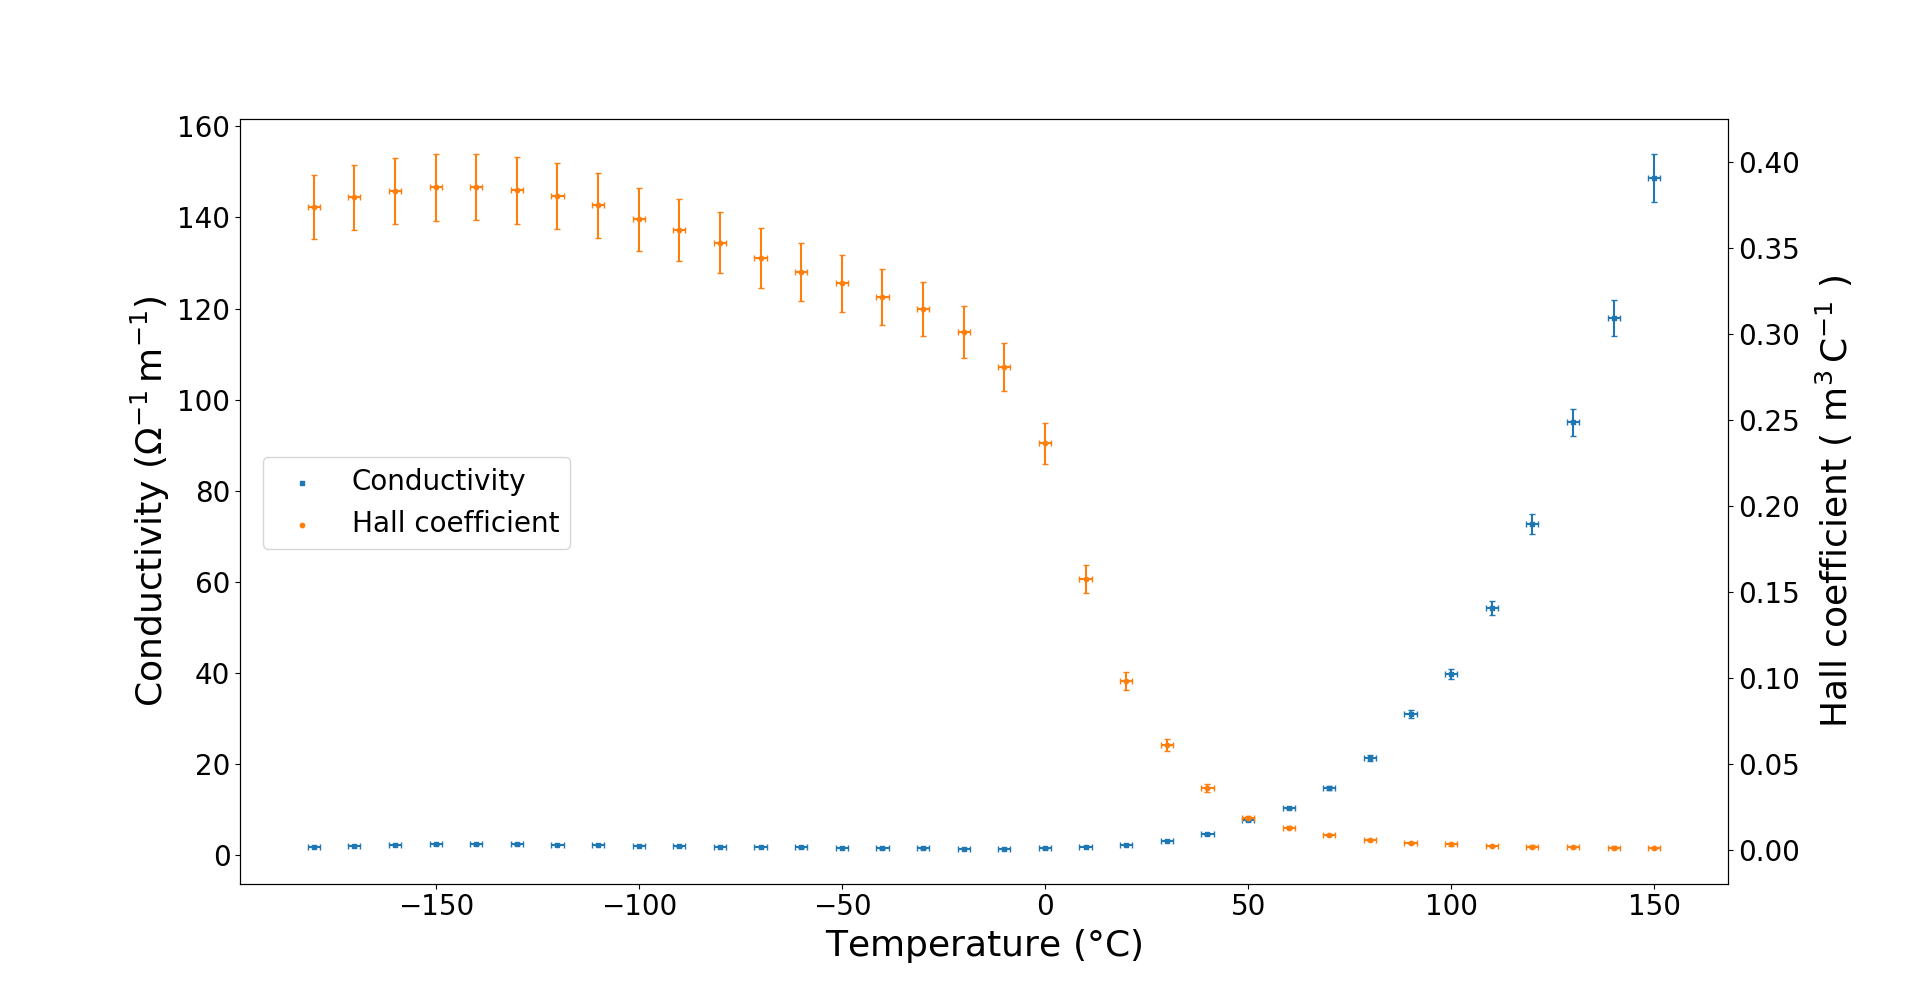
\includegraphics[height=4.2cm]{./fig/probe_A_measurement.png}
	\caption{\textbf{Messwerte Probe A}\label{fig:measurement_A}}
	\end{subfigure}
	\hfill
	\begin{subfigure}[h]{0.45\linewidth}
	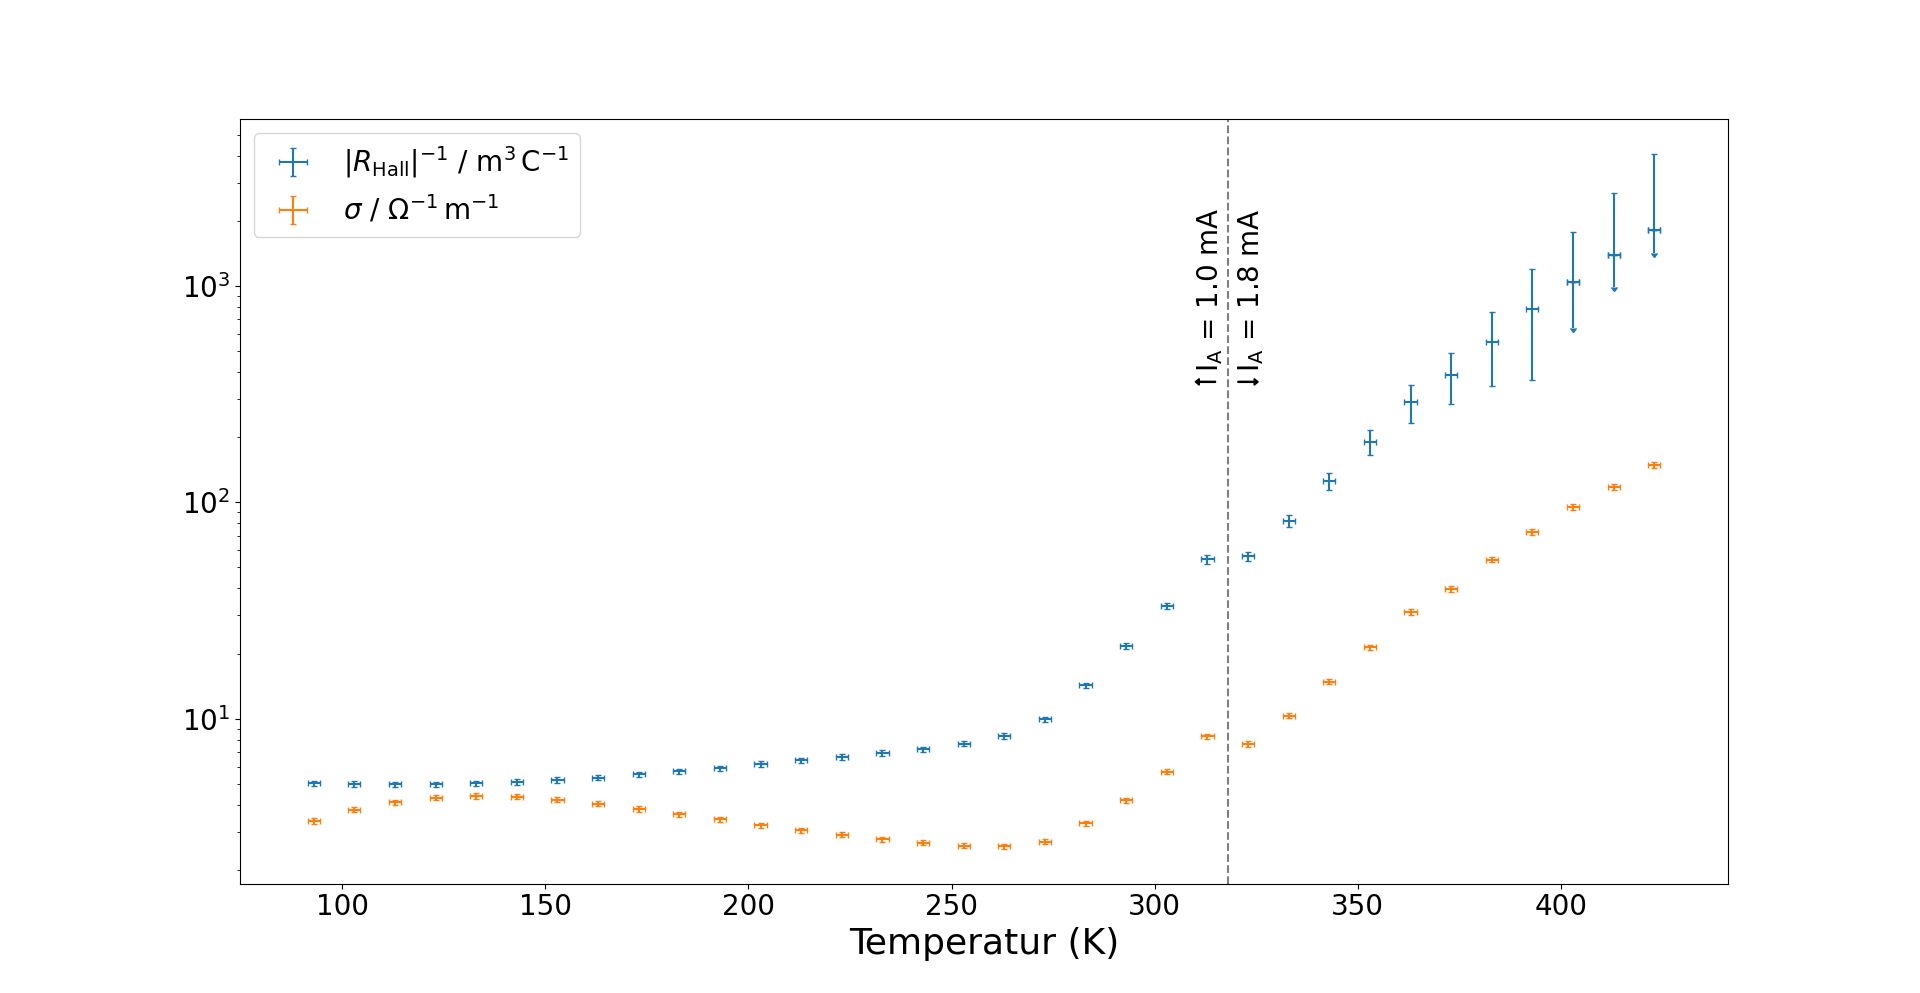
\includegraphics[height=4.2cm]{./fig/probe_A_combined_plot.png}
	\caption{\textbf{kombinierte logarithmische Darstellung}
\label{fig:logarithmic_A}}
	\end{subfigure}
	\caption*{\textbf{a)} Erkennbar ist die exponentielle Abhängigkeit der 
Leitfähigkeit $\sigma$ von der Temperatur $T$. Während der Hallkoeffizient für tiefe
Temperaturen betragsmäßig groß ist nimmt der Effekt für große Temperaturen ab. 
\textbf{b)} Logarithmische Darstellung der Messwerte. Der extrinsiche Bereich 
befindet sich um \SI{200}{\kelvin}, der intrinsische oberhalb von \SI{350}{\kelvin} 
\label{measurements_A}}
\end{figure}


